\chapter{Theory}
\label{chap:theory}

The approach of using graphs and graph theory to model networks is abundant in many areas of sciences, ranging from engineering to biology \cite{network_science_chap1}. From the perspective of machine learning, there exists many graph related tasks, with two common ones being \textit{graph classification} and \textit{node classification} \cite{quadratic_graph_classification, active_learning_node_classification}. In graph classification, the task is to classify a graph as belonging to one of several classes, whilst in node classification the task is to classify each node in the graph individually. These two problems can be generalised to graph and node regression, with the aim of predicting a continuous variable instead of a class. Graph and node classification/regression will in the remainder of the thesis be referred to as graph and node prediction. 
% From the perspective of machine learning, there exists many applications, with two common ones being \textit{graph classification} and \textit{node classification}
%% TODO TIKZ
% \begin{center}
%     \resizebox {\textwidth} {!} {
%         

\tikzset{every picture/.style={line width=0.75pt}} %set default line width to 0.75pt        

\begin{tikzpicture}[x=0.75pt,y=0.75pt,yscale=-1,xscale=1]
%uncomment if require: \path (0,208); %set diagram left start at 0, and has height of 208

%Straight Lines [id:da08555474507907834] 
\draw [color={rgb, 255:red, 155; green, 155; blue, 155 }  ,draw opacity=1 ][line width=1.5]    (144.81,72.72) -- (139.59,141.54) ;
%Straight Lines [id:da7854957979705237] 
\draw [color={rgb, 255:red, 155; green, 155; blue, 155 }  ,draw opacity=1 ][line width=1.5]    (144.81,72.72) -- (170.94,112.87) ;
%Straight Lines [id:da5355133218247532] 
\draw [color={rgb, 255:red, 155; green, 155; blue, 155 }  ,draw opacity=1 ][line width=1.5]    (139.59,141.54) -- (170.94,112.87) ;
%Straight Lines [id:da7379744038533278] 
\draw [color={rgb, 255:red, 155; green, 155; blue, 155 }  ,draw opacity=1 ][line width=1.5]    (197.06,72.72) -- (170.94,112.87) ;
%Straight Lines [id:da3385355935149281] 
\draw [color={rgb, 255:red, 155; green, 155; blue, 155 }  ,draw opacity=1 ][line width=1.5]    (197.06,72.72) -- (259.74,84.19) ;
%Straight Lines [id:da6697105472921161] 
\draw [color={rgb, 255:red, 155; green, 155; blue, 155 }  ,draw opacity=1 ][line width=1.5]    (197.06,72.72) -- (223.18,107.13) ;
%Straight Lines [id:da44213623412323666] 
\draw [color={rgb, 255:red, 155; green, 155; blue, 155 }  ,draw opacity=1 ][line width=1.5]    (249.3,135.81) -- (197.06,147.28) ;
%Straight Lines [id:da340514368127399] 
\draw [color={rgb, 255:red, 155; green, 155; blue, 155 }  ,draw opacity=1 ][line width=1.5]    (223.18,107.13) -- (249.3,135.81) ;
%Straight Lines [id:da07640316595483987] 
\draw [color={rgb, 255:red, 155; green, 155; blue, 155 }  ,draw opacity=1 ][line width=1.5]    (259.74,84.19) -- (249.3,135.81) ;
%Shape: Trapezoid [id:dp2008857707852969] 
\draw  [color={rgb, 255:red, 255; green, 255; blue, 255 }  ,draw opacity=1 ][fill={rgb, 255:red, 255; green, 255; blue, 255 }  ,fill opacity=1 ] (254.52,89.93) -- (257.66,78.46) -- (261.83,78.46) -- (264.97,89.93) -- cycle ;
%Image [id:dp4810218304838956] 
\draw (259.74,84.19) node  {\includegraphics[width=15.67pt,height=17.2pt]{ClbFhBFF8L-person-blue-36dp-filled.svg}};

%Straight Lines [id:da17683212694460426] 
\draw [color={rgb, 255:red, 155; green, 155; blue, 155 }  ,draw opacity=1 ][line width=1.5]    (139.59,141.54) -- (197.06,147.28) ;
%Shape: Trapezoid [id:dp06527551163848622] 
\draw  [color={rgb, 255:red, 255; green, 255; blue, 255 }  ,draw opacity=1 ][fill={rgb, 255:red, 255; green, 255; blue, 255 }  ,fill opacity=1 ] (191.83,153.01) -- (194.97,141.54) -- (199.15,141.54) -- (202.28,153.01) -- cycle ;
%Image [id:dp24121370862546265] 
\draw (197.06,147.28) node  {\includegraphics[width=15.67pt,height=17.2pt]{ClbFhBFF8L-person-blue-36dp-filled.svg}};

%Shape: Trapezoid [id:dp6568478256577734] 
\draw  [color={rgb, 255:red, 255; green, 255; blue, 255 }  ,draw opacity=1 ][fill={rgb, 255:red, 255; green, 255; blue, 255 }  ,fill opacity=1 ] (134.37,147.28) -- (137.5,135.81) -- (141.68,135.81) -- (144.81,147.28) -- cycle ;
%Image [id:dp6219332582048571] 
\draw (139.59,141.54) node  {\includegraphics[width=15.67pt,height=17.2pt]{ClbFhBFF8L-person-blue-36dp-filled.svg}};

%Straight Lines [id:da3735509406273694] 
\draw [color={rgb, 255:red, 155; green, 155; blue, 155 }  ,draw opacity=1 ][line width=1.5]    (170.94,112.87) -- (223.18,107.13) ;
%Shape: Trapezoid [id:dp8065935750477351] 
\draw  [color={rgb, 255:red, 255; green, 255; blue, 255 }  ,draw opacity=1 ][fill={rgb, 255:red, 255; green, 255; blue, 255 }  ,fill opacity=1 ] (217.95,112.87) -- (221.09,101.4) -- (225.27,101.4) -- (228.4,112.87) -- cycle ;
%Image [id:dp45354658145120497] 
\draw (223.18,107.13) node  {\includegraphics[width=15.67pt,height=17.2pt]{ClbFhBFF8L-person-blue-36dp-filled.svg}};

%Straight Lines [id:da3264902727456349] 
\draw [color={rgb, 255:red, 155; green, 155; blue, 155 }  ,draw opacity=1 ][line width=1.5]    (249.3,135.81) -- (170.94,112.87) ;
%Shape: Trapezoid [id:dp866311010615511] 
\draw  [color={rgb, 255:red, 255; green, 255; blue, 255 }  ,draw opacity=1 ][fill={rgb, 255:red, 255; green, 255; blue, 255 }  ,fill opacity=1 ] (244.07,141.54) -- (247.21,130.07) -- (251.39,130.07) -- (254.52,141.54) -- cycle ;
%Image [id:dp8422386634219512] 
\draw (249.3,135.81) node  {\includegraphics[width=15.67pt,height=17.2pt]{ClbFhBFF8L-person-blue-36dp-filled.svg}};

%Shape: Trapezoid [id:dp8073086406080059] 
\draw  [color={rgb, 255:red, 255; green, 255; blue, 255 }  ,draw opacity=1 ][fill={rgb, 255:red, 255; green, 255; blue, 255 }  ,fill opacity=1 ] (165.71,118.6) -- (168.85,107.13) -- (173.02,107.13) -- (176.16,118.6) -- cycle ;
%Image [id:dp888581341362926] 
\draw (170.94,112.87) node  {\includegraphics[width=15.67pt,height=17.2pt]{ClbFhBFF8L-person-blue-36dp-filled.svg}};

%Straight Lines [id:da4374734471484929] 
\draw [color={rgb, 255:red, 155; green, 155; blue, 155 }  ,draw opacity=1 ][line width=1.5]    (144.81,72.72) -- (197.06,72.72) ;
%Shape: Trapezoid [id:dp17137240691479927] 
\draw  [color={rgb, 255:red, 255; green, 255; blue, 255 }  ,draw opacity=1 ][fill={rgb, 255:red, 255; green, 255; blue, 255 }  ,fill opacity=1 ] (191.83,78.46) -- (194.97,66.99) -- (199.15,66.99) -- (202.28,78.46) -- cycle ;
%Image [id:dp3965566139299834] 
\draw (197.06,72.72) node  {\includegraphics[width=15.67pt,height=17.2pt]{ClbFhBFF8L-person-blue-36dp-filled.svg}};

%Shape: Trapezoid [id:dp7022737407670283] 
\draw  [color={rgb, 255:red, 255; green, 255; blue, 255 }  ,draw opacity=1 ][fill={rgb, 255:red, 255; green, 255; blue, 255 }  ,fill opacity=1 ] (139.59,78.46) -- (142.72,66.99) -- (146.9,66.99) -- (150.04,78.46) -- cycle ;
%Image [id:dp7793647929632923] 
\draw (144.81,72.72) node  {\includegraphics[width=15.67pt,height=17.2pt]{ClbFhBFF8L-person-blue-36dp-filled.svg}};


%Rounded Rect [id:dp2921184592491468] 
\draw   (120,74) .. controls (120,60.75) and (130.75,50) .. (144,50) -- (250.11,50) .. controls (263.37,50) and (274.11,60.75) .. (274.11,74) -- (274.11,146) .. controls (274.11,159.25) and (263.37,170) .. (250.11,170) -- (144,170) .. controls (130.75,170) and (120,159.25) .. (120,146) -- cycle ;

%Straight Lines [id:da280482111384722] 
\draw    (474,110) -- (414,110) ;
%Rounded Rect [id:dp23949785762119213] 
\draw   (324.11,92) .. controls (324.11,85.37) and (329.48,80) .. (336.11,80) -- (402.11,80) .. controls (408.74,80) and (414.11,85.37) .. (414.11,92) -- (414.11,128) .. controls (414.11,134.63) and (408.74,140) .. (402.11,140) -- (336.11,140) .. controls (329.48,140) and (324.11,134.63) .. (324.11,128) -- cycle ;

%Straight Lines [id:da18593803425726807] 
\draw    (324.11,110) -- (274.11,110) ;
%Rounded Rect [id:dp14732801608712798] 
\draw   (474,98) .. controls (474,93.58) and (477.58,90) .. (482,90) -- (576,90) .. controls (580.42,90) and (584,93.58) .. (584,98) -- (584,122) .. controls (584,126.42) and (580.42,130) .. (576,130) -- (482,130) .. controls (477.58,130) and (474,126.42) .. (474,122) -- cycle ;
%Image [id:dp556169067273697] 
\draw (45.6,68) node  {\includegraphics[width=30pt,height=30pt]{ClbFhBFF8L-person-blue-36dp-filled.svg}};
%Image [id:dp2790482390271307] 
\draw (45.6,108) node  {\includegraphics[width=30pt,height=30pt]{ClbFhBFF8L-person-blue-36dp-filled.svg}};
%Image [id:dp9089881134245916] 
\draw (45.6,148) node  {\includegraphics[width=30pt,height=30pt]{ClbFhBFF8L-person-blue-36dp-filled.svg}};
%Rounded Rect [id:dp06427479999848584] 
\draw  [dash pattern={on 4.5pt off 4.5pt}] (12,61.6) .. controls (12,54.09) and (18.09,48) .. (25.6,48) -- (66.4,48) .. controls (73.91,48) and (80,54.09) .. (80,61.6) -- (80,156.4) .. controls (80,163.91) and (73.91,170) .. (66.4,170) -- (25.6,170) .. controls (18.09,170) and (12,163.91) .. (12,156.4) -- cycle ;
%Straight Lines [id:da8499548057058206] 
\draw    (120,110) -- (80,110) ;

% Text Node
\draw (340.11,96) node [anchor=north west][inner sep=0.75pt]   [align=left] {{\Large Model}};
% Text Node
\draw (439,89.4) node [anchor=north west][inner sep=0.75pt]    {$y$};
% Text Node
\draw (295.11,90.4) node [anchor=north west][inner sep=0.75pt]    {$X$};
% Text Node
\draw (483,99) node [anchor=north west][inner sep=0.75pt]   [align=left] {{\large Predictions}};


\end{tikzpicture}

%     }
% \end{center}

\begin{figure}[H]
    \centering
        \begin{subfigure}{.5\textwidth}
            \centering
            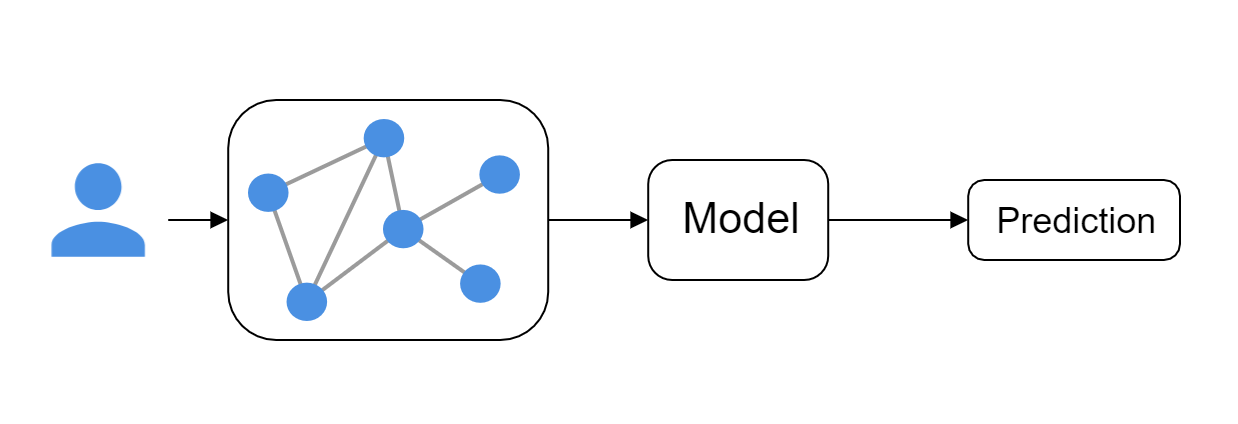
\includegraphics[width=1\linewidth]{chapters/images_theory/graph_classification.png}
            \caption{Graph classification}
            \label{fig:subject_prediction}
        \end{subfigure}%
        \begin{subfigure}{.5\textwidth}
            \centering
            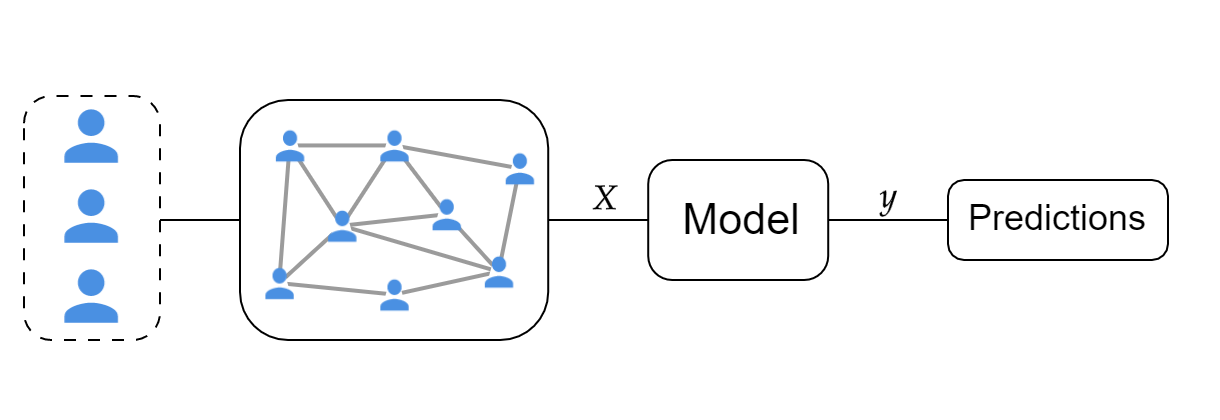
\includegraphics[width=1\linewidth]{chapters/images_theory/node_classification.png}
            \caption{Node classification}
            \label{fig:population_prediction}
        \end{subfigure}
    \caption{Schematic representations of graph and node classification.}
    \label{fig:graph_and_node_class}
\end{figure}

In the context of neuroscience, graph and node prediction may correspond to predicting some property of a subject, for instance sex or age. Graph prediction is relevant when each subject is associated with a graph, which in this thesis will correspond to the functional networks in a subjects brain. A schematic visualisation of graph prediction can be seen in figure \ref{fig:subject_prediction}. It is also possible to introduce the concept of \textit{population graphs}, where each node represents a single subject, in which node prediction would become relevant. See figure \ref{fig:population_prediction} for a representation of node prediction in population graphs. 

% In this chapter, the foundations of graph theory, graph convolutional neural networks and explainability methods will be presented. The chapter begins with a primer on general graph theory, followed by the description of two specific types of graphs, population and multiplex graphs. Next, graph convolutional neural networks will be presented, followed by a black-box analysis methods known as Zorro. The chapter will be concluded with a brief overview of related works regarding GCNs and explainability of AI. 

% The remainder of the chapter will present a theoretical background for graphs, graph convolutional neural networks and explaiability for AI. Specifically, 

% Graph prediction is relevant when each subject is associated with a graph, and can be schematically visualised in figure \ref{fig:subject_prediction}. An example of such a graph could be the functional networks in a subjects brain.

% In this chapter, the necessary theory of graphs, graph convolutional neural networks and explaiability for AI will be presented.


% The following of this chpter will aim to present necceccary theory for performing maching leaning on graphs, both 

% In this thesis, two kinds of graphs will be considered: subject-specific graphs for graph prediction, and population graphs for node prediction. The subject-specific graphs will represent the functional brain networks for each subject, and will be formulated as a specific kind of graph known as a multiplex graph. 

\section{General graph theory}
\label{sec:general_graph_theory}

Let $\mathcal{G}$ be a graph, associated with a set of nodes $V$ and a set of edges $E$. The edges forms the connections between nodes, and for a pair of nodes $(i,j)$ the corresponding edge may be denoted $e_{ij}$. The neighbours $N(v)$ to a certain node $v \in V$ are defined as the nodes $u \in V$ that are connected to $v$, $e_{vu} \neq 0$. Each node $v$ may also be associated with \textit{node features}, $x_v$. $x_v$ may represent some state of or information about node $v$, which in practice can take the form of a vector of numbers \cite{active_learning_node_classification}.
% in applications typically takes the form of a number, a vector of numbers, or a piece of text etc

A graph $\mathcal{G}$ is considered to be \textit{undirected} if all edges in the graph are undirected, $e_{ij} \equiv e_{ji}$, and \textit{directed} if all edges are directed, $e_{ij} \not\equiv e_{ji}$. The edges in $\mathcal{G}$ may be succinctly summarised in an \textit{adjacency matrix} $A$ defined as
\begin{equation}
    A_{ij} = \begin{cases} \mbox{1,} & \mbox{if } e_{ij} \in E \\ \mbox{0,} & \mbox{otherwise.} \end{cases}
    \label{eq:adjacencydefinition}
\end{equation}
From definition \eqref{eq:adjacencydefinition} it follows that undirected graphs have a symmetric adjacency matrix, $A_{ij} = A_{ji}$. From the adjacency matrix, the degree matrix $D$ is defined as
\begin{equation}
    D_{ij} = \begin{cases} \sum_j A_{ij}, & \mbox{if } i = j \\ \mbox{0,} & \mbox{otherwise,} \end{cases}
    \label{eq:degreematrixdefinition}
\end{equation}
which describes each node's \textit{degree}, the number of edges connected to each node.

Moreover, each edge in $\mathcal{G}$ may be associated with a weight $w_{ij}$, and $\mathcal{G}$ is then denoted as a \textit{weighted} graph. The adjacency matrix becomes $A_{ij} = w_{ij}$, and the degree matrix now describes the \textit{strength} of each node, which is defined as the sum of the weights of all edges connected to the node. Weights in a weighted graph may be interpreted differently depending on the application \cite{adventures_in_graph_theory_chap1}. They can be seen as the connection strength between devices in a cellular network, the cost of a ticket along a route in a train network, the flow of goods in a logistics setting etc. All graphs referenced in the remainder of the thesis will be weighted and undirected unless otherwise specified.

\section{Population graphs and multiplex graphs}
\label{sec:similarity_measure}

In a population graph, each node corresponds to an individual, and the edges relate all individuals to each other. One way of calculating the weights of the population graph is by using a similarity measure. The similarity measure greatly shapes the resulting population graph, and should be chosen with the specific application in mind. One common approach is to define a similarity measure $\sigma$ as a distance measure $D$ inverted by a kernel $K$. The similarity measure between two data points $x_1$ and $x_2$ may then be written as
\begin{equation}
    \sigma(x_1,x_2) = K \left(D\left(x_1, x_2\right) \right).
    \label{eq:similarity_measure}
\end{equation}

\begin{figure}[H]
    \centering
    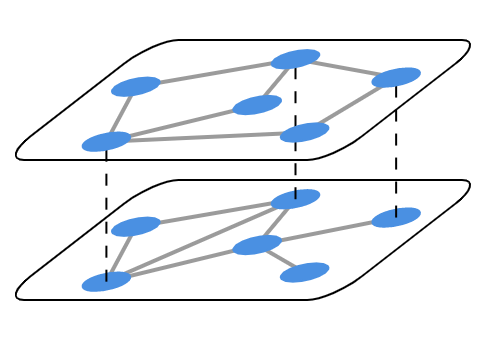
\includegraphics[width=0.7\textwidth]{chapters/images_theory/multiplex.png}
    \caption{An example of a two-layered multiplex graph, with the same nodes in each layer but different edges.}
    \label{fig:multiplex_graph}
\end{figure}
Another type of graph relevant for this thesis is a multiplex graph. A multiplex graph is a layered graph where each layer can represent a different type of interaction between nodes \cite{multiplex_book_chap2}. One example of a multiplex graph with the same nodes in all layers is a graph with cities as nodes and different means of transportation as edges. Edges representing highways and railways makes up two different graphs, but they might be combined into a multiplex graph since they share the same nodes, the cities. See figure \ref{fig:multiplex_graph} for a visual representation of a two-layered multiplex graph, in which the nodes are fixed, but the edges are different in each layer.

\section{Graph Convolutional Neural Networks}
\label{sec:gcn}

Graph Convolutional Neural Networks (GCNs) are a class of neural networks that generalize the notion of convolutions from grid data to graph structured data \cite{wu_review}. Regular convolutional operations operate on structured grids of data, for instance the pixels in an image, where each grid point is only connected to its adjacent neighbours. This may not be the case for graph structured data, where any pair of nodes can be connected. Generalizing the convolutional operator to the graph domain enables a GCN to utilize information about the graph structure, in the same way a regular CNN can utilize information about structures in e.g. an image \cite{wu_review}.

The theoretical foundations for GCNs will be explained in three parts. First, the concept of convolutions in the graph domain, and how they are implemented in a computationally efficient manner. Then, a layer-wise propagation rule for a graph convolutional layer based on the implementation of convolutions, and finally a heuristic interpretation known as \textit{message passing}.

\subsection{Efficient convolutions in the graph domain}

Let $\mathcal{G}$ be an undirected graph, with $N$ nodes and adjacency matrix $A$. The graph Laplacian $L$ is defined as $L=D-A$, and may be normalized according to
\begin{equation}
    L_\text{norm} = D^{-1/2} L D^{-1/2} =  I_N - D^{-1/2} A D^{-1/2},
    \label{eq:normalized_graph_laplacian}
\end{equation}
where $I_N$ is the $N \times N$ identity matrix. With $L = L_{\text{norm}}$, the convolution of a signal $x \in R^N$ defined on the nodes of $\mathcal{G}$ with a filter $g_\theta = diag(\theta)$, parametrized by $\theta \in R^N$, can in the Fourier domain be written as
\begin{equation}
    g_\theta * x = U g_\theta U^T x,
    \label{eq:graph_convolution}
\end{equation}
where $U$ is an orthogonal matrix containing the eigenvectors of $L$ \cite{kipf_semi_supervised}. Performing convolutions using equation \ref{eq:graph_convolution} may however be computationally intractable in practice, partly because multiplication with $U$ is $\mathcal{O}(N^2)$ and partly because calculating $U$ requires the eigendecomposition of $L$, which may be very computationally expensive for large graphs \cite{kipf_semi_supervised}. Kipf et al. \cite{kipf_semi_supervised} proposes a solution to this problem, in which the convolution is approximated with an expansion in Chebyshev polynomials $T_k(x)$:s,
\begin{equation}
    g_{\theta'} * x \approx \sum_{k=0}^K \theta'_k T_k(\tilde{L})x,
    \label{eq:convolution_approximation}
\end{equation}
where $\tilde{L} =  \frac{2}{\lambda_{\text{max}}}L - I_N$, and $\lambda_{\text{max}}$ is the largest eigenvalue of $L$. $\theta'_k$ is here a vector of Chebyshev coefficients, which in the context of machine learning corresponds to trainable parameters. The interpretation of equation \eqref{eq:convolution_approximation} is that the convolution is $K^{\text{th}}$ order local, i.e. that a convolution considers each node and their $K^{\text{th}}$ order neighbors, the neighbours that are at most $K$ steps away in the graph. 

\subsection{Layer-wise propagation rule}
By setting $K = 1$ and a single trainable parameter $\theta = \theta_0' = -\theta_1'$ the convolution in equation \eqref{eq:convolution_approximation} can according to \cite{kipf_semi_supervised} be further simplified as 
\begin{equation}
    g_{\theta'} * x \approx \theta \left(I_N + D^{-1/2}AD^{-1/2} \right)x. 
    \label{eq:k1_approximation_step3}
\end{equation}
Setting $K=1$ limits the convolution to only consider a node ($k=0$) and its closest neighbours ($k=1$). Implementing convolutions as in equation \eqref{eq:k1_approximation_step3} may however lead to exploding or vanishing gradients, since the eigenvalues of $I_N + D^{-1/2}AD^{-1/2}$ lies in the range $[0, 2]$. This problem can be avoided using a \textit{renormalization trick}:
\begin{equation}
    I_N + D^{-1/2}AD^{-1/2} \rightarrow \tilde{D}^{-1/2} \tilde{A} \tilde{D}^{-1/2}
    \label{eq:renormalization_trick}
\end{equation}
where $\tilde{A} = A + I_N$ and $\tilde{D} = \sum_j \tilde{A}_{ij}$.

The convolutional operation may now be generalized to a signal $X \in \mathbb{R}^{N \times C}$, defined on the $N$ nodes of the graph and with a $C$-dimensional feature vector for each node. The signal $X$ thus has $C$ input channels. Furthermore, let the convolution apply $F$ filters to the $C$ input channels. The application of such a convolution can thus be written

\begin{equation}
    Z = \tilde{D}^{-1/2} \tilde{A} \tilde{D}^{-1/2} X \Theta,
    \label{eq:propagation_rule}
\end{equation}
with $\Theta \in \mathbb{R}^{C\times F}$ being a matrix of filter parameters and $Z \in \mathbb{R}^{N\times F}$ as the convolved signal. This propagation rule in equation \eqref{eq:propagation_rule}, when paired with an activation function $\sigma$ such that $H = \sigma\left(Z \right)$, forms the basis for a GCN. 

Recall that in order to arrive at equation \eqref{eq:propagation_rule}, the Chebyshev polynomial expansion in equation \eqref{eq:convolution_approximation} was truncated at $K=1$. By truncating the Chebyshev polynomial, the convolution operator only considers each node and its closest neighbours, and becomes a linear function in $L$. These two points may seem to be limitations in the representational strength of the graph convolutional layer, however this is not necessarily the case \cite{kipf_semi_supervised}. First, larger neighbourhoods can be convolved over by stacking multiple layers, with the first layer considering a node and its neghbours, the second layer considering the neighbours neighbours and so on. Secondly, keeping the representation linear in $L$ actually makes it more flexible, since it is not dependant on the explicit parametrization given by the Chebyshev polynomials \cite{kipf_semi_supervised}. Combined, a deep GCN consisting of several stacked graph convolutional layers paired with possibly non-linear activation functions $\sigma$ can still model a rich class of convolutional filter functions, whilst keeping computational costs low. 


\subsection{Message passing interpretation for GCNs}
\label{subsec:message_passing}

Heuristically, a graph convolutional layer can be seen to perform a sort of \textit{message passing}, in that each node receives messages (aggregates features) from all of its closest neighbours. This can be seen by studying the propagation rule in equation \eqref{eq:propagation_rule} for a single node $i$, a single feature channel $C=1$ and a single filter channel $F=1$, and explicitly rewriting it as a sum:
\begin{equation}
    z_i = \theta \left(\left(\tilde{D}^{-1/2} \tilde{A} \tilde{D}^{-1/2}\right)_{ii} x_{i} + \sum_{j \neq i} \left(\tilde{D}^{-1/2} \tilde{A} \tilde{D}^{-1/2}\right)_{ij} x_{j} \right) = \theta \left(h_{ii} + \sum_{j \neq i} h_{ij} \right).
\end{equation}
$z_i$ and $x_i$ corresponds to the activation and feature for node $i$, respectively. $h_{ij}$ can be interpreted as a normalized message, communicating the state $x_j$ weighted by the normalized connection between node $j$ and $i$. The activation $z_i$ can then be seen as an aggregation of normalized messages from all neighbouring nodes, $h_{ij}$, and itself, $h_{ii}$. See figure \ref{fig:message_passing} for a visual representation of how the messages are passed to node $i$ from it's neighbours. In this manner information can flow through the graph, and by stacking multiple graph convolutional layers the information can spread over successively larger neighbourhoods. With the message passing interpretation, a deep GCN can be seen to draw upon the informational flow patterns in the graph. This enables it to learn from the graph structure, similarly to how a deep CNN can extract information from structures in an image.

\begin{figure}[H]
    \centering
    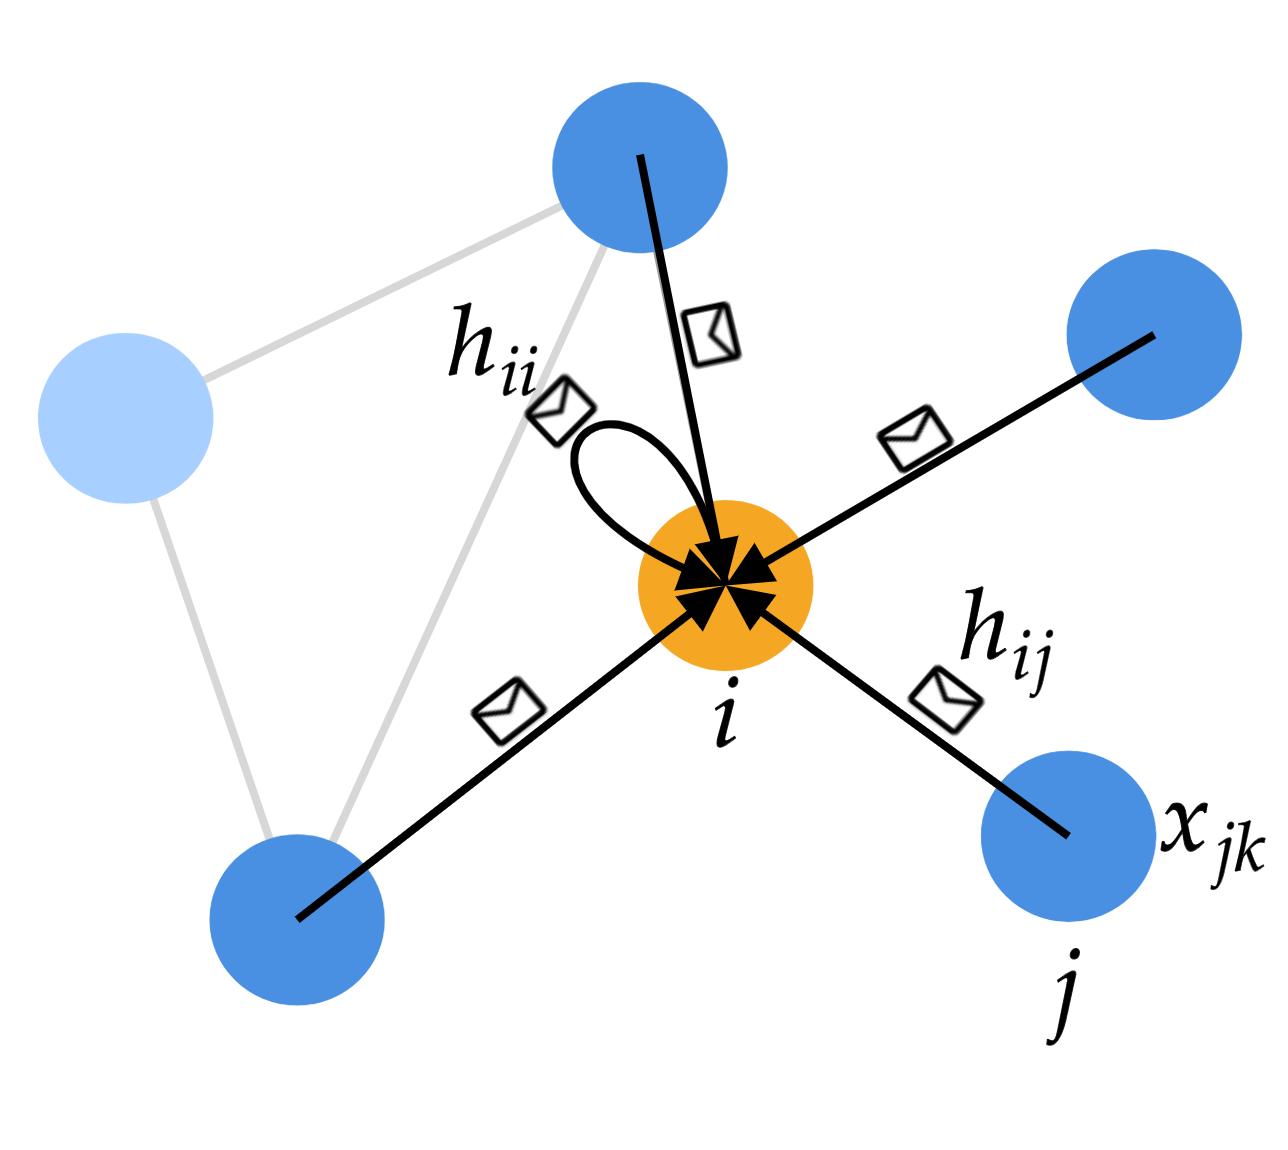
\includegraphics[width=0.5\linewidth]{chapters/images_theory/message_passing.png}
    \caption{A schematic representation of the message passing interpretation of a graph convolutional layer. The messages $h_{ij}$ are sent from node $j$ to node $i$.}
    \label{fig:message_passing}
\end{figure}




\section{Zorro -- an algorithm for explainability in GCNs}
\label{sec:zorro}
% To describe the Zorro algorithm

Zorro is an algorithm for determining which nodes and features are important for a trained GCN model performing node classification on a graph with adjacency matrix $A$ and feature matrix $X$ \cite{zorro}. The model is denoted $\Phi_n(X,A)$ and takes $A$ and $X$ as input, and gives a prediction for a node $n$ in the graph. The general idea is to replace the feature matrix $X$ by noise and then reintroduce nodes and features to successively make the model prediction similar to the original. The reintroduced nodes $V$ and features $F$ are referred to as an explanation $\mathcal{S} = \{V, F\}$. Noise is applied to $X$ through element-wise multiplication with a masking matrix $S$ representing $\mathcal{S}$ and a matrix of random noise $Z$, according to
\begin{equation}
    Y_\mathcal{S} = X \odot S + Z \odot (1- S), \quad Z \sim \mathcal{N}.
\end{equation}
The noise distribution $\mathcal{N}$ is set to the distribution of all features in $X$. The prediction of the model $\Phi$ on the masked data is then $\Phi_n(Y_{\mathcal{S}}, A)$. To evaluate an explanation $\mathcal{S}$, i.e. if the unmasked nodes and features are important for the prediction of a specific node, the fidelity of the explanation is calculated by
\begin{equation}
    \mathcal{F}(\mathcal{S}) = \mathbb{E}_{Y_{\mathcal{S}}|Z\sim\mathcal{N}}\left[\mathbbm{1}_{\Phi_n(X,A) = \Phi_n(Y_{\mathcal{S}},A)}\right].
    \label{eq:Ys}
\end{equation}
The fidelity of an explanation is a measure of how likely it is for a model with a masked data set to give the same prediction as a model with the original data set.

For each node $n$, the algorithm begins with an empty explanation $S_n = \{\emptyset, \emptyset\}$, and thus $\Phi_n(Y_s, A)$ will have a completely random input according to equation \ref{eq:Ys}. Then, the node or feature that increases the fidelity of the explanation the most is added to the explanation. More and more nodes and features are iteratively added until the fidelity of the explanation exceeds a hyper parameter $\tau$. The resulting explanation indicates which nodes and features where important to make the prediction of node $n$. The algorithm can then be repeated for all the nodes in the graph.

\section{Similar works: the intersection of GCNs and neuroscience}

% Ta upp relaterade arbeten och knyt ihop med introduction inför metoden. E.g. Jansson sandström, stankeviciute.

There have been numerous papers published in the last few years applying graph neural networks in neuroscience with similar aims as that of this thesis; to develop and explain accurate classifiers for brain age and sex prediction. For age prediction, notable works include Stankevicuete et al. \cite{stankeviciute} and Amoroso et al. \cite{amoroso_multiplex_age}, which both utilize structural MRI data. Stankevicuete et al. applies GCNs to a population graph of subjects, and Amoroso et al. uses an ANN with graph measures as input features to predict age. The problem of sex prediction is approached in Arslan et al. \cite{arslan}, which uses GCNs, and in the work by Kim and Ye \cite{understanding_gnn}, which uses a variant of GNN known as a Graph Isomorphism Network (GIN). Both of these studies applies their models to fMRI data. Furthermore, Arslan et al. and Kim and Ye also analyses the gradients within the models, with the goal of identifying which functional brain networks are related to sex. 

What sets this thesis apart from the work in \cite{stankeviciute, amoroso_multiplex_age, arslan, understanding_gnn} is threefold: Firstly, resting-state fMRI data is used for age prediction. Secondly, relevant functional brain networks for age prediction are investigated. Finally, the relevant functional brain networks are mapped using Zorro, a new method for analysing black-box models.

% Another relevant publication for this specific thesis is the Master Thesis by Jansson and Sandström \cite{jansson_sandstrom}, in which the applications of GCNs in neuroscience where explored and applied on the problem of classifying Alzheimer's Disease based on MRI data. The thesis by Jansson and Sandström is the precursor to this very thesis, and it's their interesting findings that motivated this master thesis project. 
